Complex structures in nature are often composed of elementary pieces that obey simple local composition rules. Molecular biology, nanomanufacturing, and self-assembly are prime examples. Mathematical models for this phenomenon typically rely on rigidity theory and formal languages. In this paper, we study the realizability of complex structures that are given with a local specification. We consider two models in Euclidean plane.

\begin{enumerate}
\item A \textbf{polygonal linkage} is a set $\PP$ of convex polygons, and a set $\HH$ of hinges,
where each hinge $h\in \HH$ corresponds to two points on the boundary of two distinct polygons.
A \emph{realization} of a polygonal linkage is an interior-disjoint placement of congruent copies of the polygons in $\PP$ such that the points corresponding to each hinge are identified (Fig.~\ref{fig:1}, left).
\item A \textbf{disk arrangement} is a set $\DD$ of pairwise interior-disjoint disks in the plane. The contact graph of a disk arrangement $\DD$ is a graph $G=(\DD,E)$ where two vertices are adjacent if the corresponding disks intersect (kiss). A \emph{realization} of a vertex-weighted graph $G$ as a contact graph of disks is a disk arrangement whose contact graph is $G$ and the radius of each disk is the corresponding vertex weight.
\end{enumerate}
\begin{figure}[htbp]
  \centering
 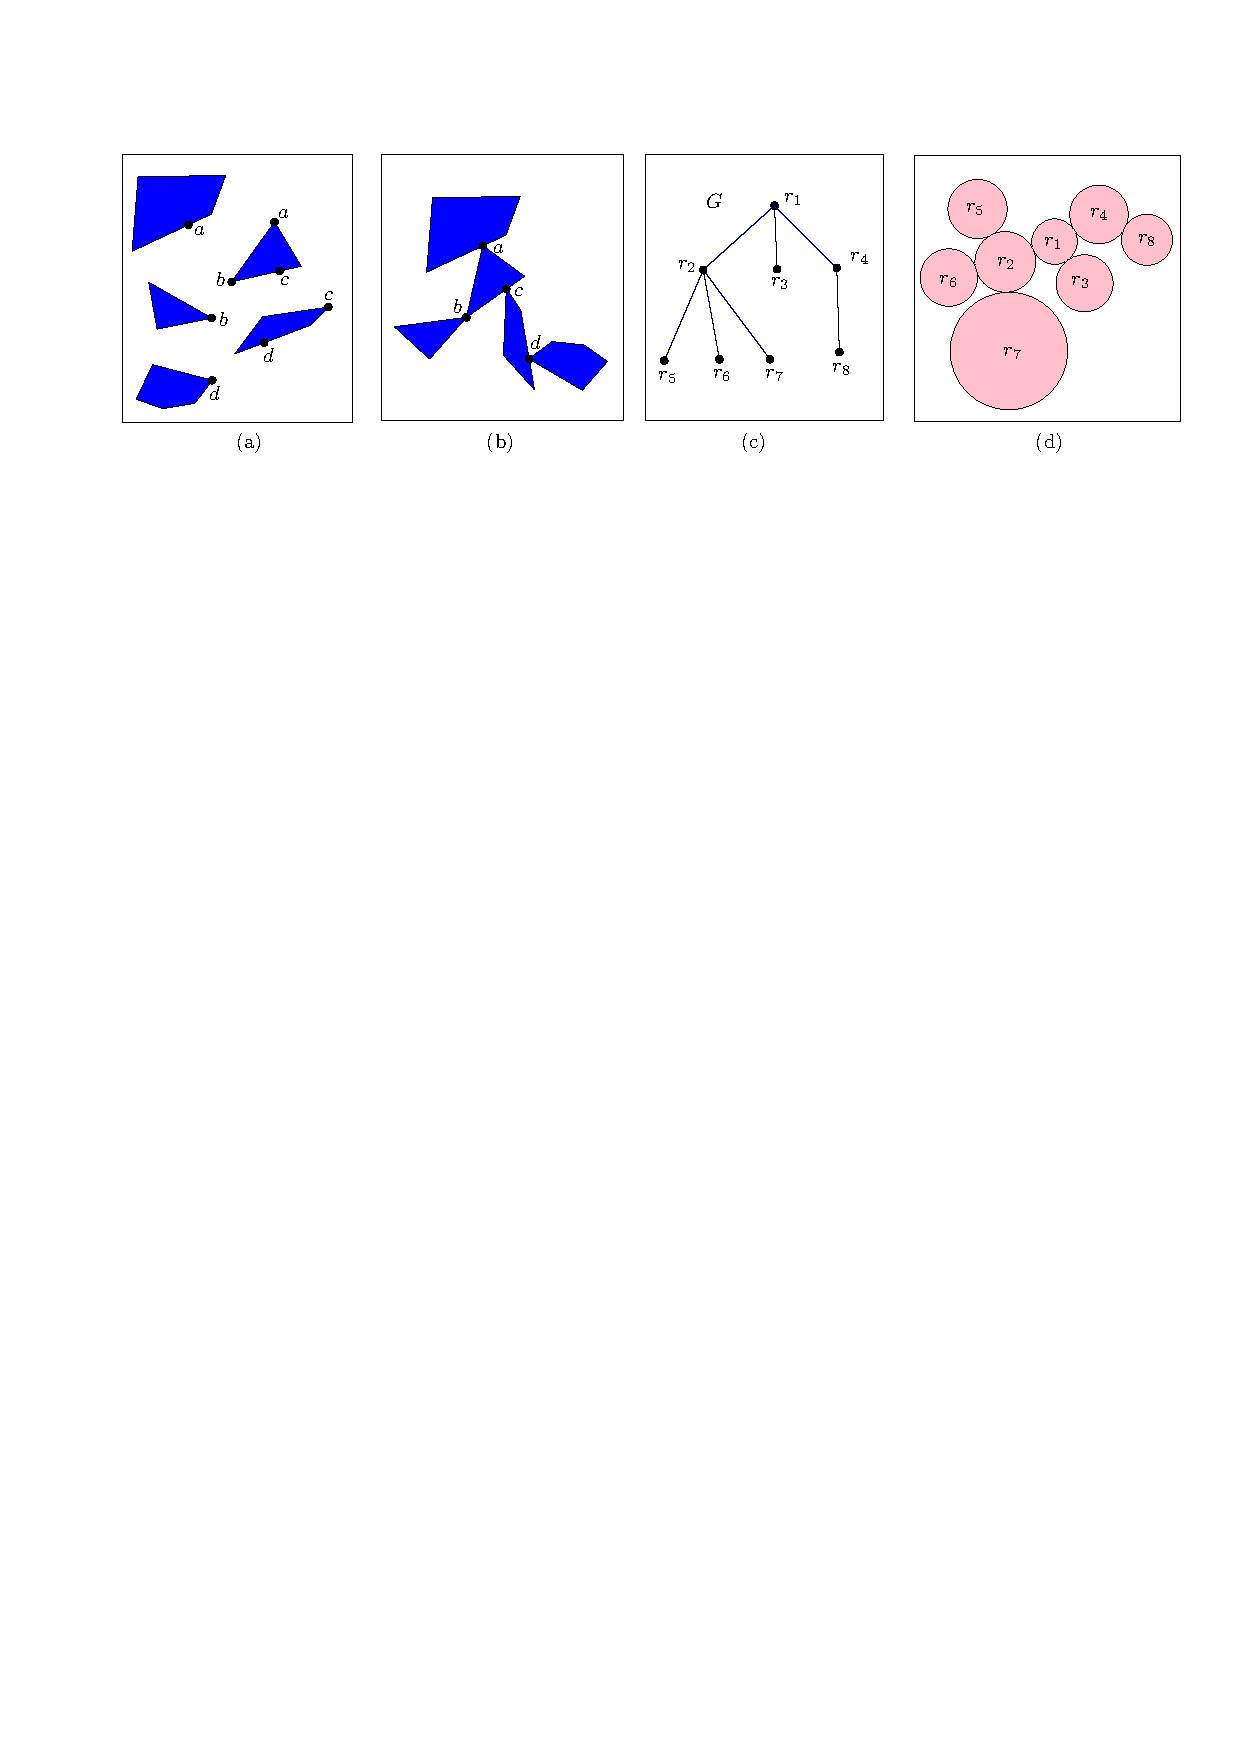
\includegraphics[width=0.95\textwidth]{graphics/fig1}
\caption{\small (a) A set of convex polygons and hinges. (b) A realization of the polygonal linkage from (a).
(c) A graph $G$ with vertex weights $r_1,\ldots, r_8$. (d) A disk arrangement that realizes the 
weighted graph $G$ as a contact graph with radii equal to the corresponding weights.}
  \label{fig:1}
\end{figure}
Each model has two variants, depending on whether \emph{reflection} is allowed for the realization of each piece independently. For polygonal linkages, an \emph{oriented realization} requires translated and rotated copies of the polygons in $\PP$ (i.e., reflection is not allowed). An \emph{ordered contact graph} for a disk arrangement is a \emph{plane graph} $G$, where the circular order of the neighbors of each vertex is specified, and an \emph{oriented realization} is disk arrangement with the given ordered contact graph.


\smallskip\noindent{\bf Related Previous Work.}
Polygonal linkages (or body-and-joint frameworks) are a generalization of classical linkages (bar-and-joint frameworks) in rigidity theory. A linkage is a graph $G=(V,E)$ with given edge lengths. A realization of a linkage is a (crossing-free) straight-line embedding of $G$ in the plane.
Bhatt and Cosmadakis~\cite{BC87} proved that the realizability of linkages is NP-hard.
Their ``logic engine'' method~\cite{SFM+11,BET+99,FHW97,HK01}, has become a powerful tool in graph drawing.
The logic engine is a graph composed of rigid 2-connected components, connected by cut vertices (hinges). The two possible realizations of each 2-connected component (that differ by a single reflection)  represent the truth assignment of a binary variable. This method does not applicable to the \emph{oriented} version of the realizability, where the circular order of the neighbors of each vertex is part of the input. Cabello et al.~\cite{CDR07,EW90} proved that the realizability of 3-connected linkages (where the orientation is unique by Steinitz's theorem) is NP-hard, but efficiently decidable for near-triangulations~\cite{CDR07,BV96}.

Note that every \emph{tree} linkage can be realized in $\RR^2$ (with almost collinear edges). According to the celebrated \emph{Carpenter's Rule Theorem}~\cite{CDR03,Str05}, every realization of a path (or a cycle) linkage can be continuously moved (without self-intersection) to any other realization. In other words, the realization space of such a linkage is always connected. However, there are trees of maximum degree 3 with at few as 8 edges whose realization space is disconnected~\cite{BCD+09}; and deciding whether the realization space of a tree linkage
is connected is PSPACE-complete~\cite{AKR+04}. (Earlier, Reif~\cite{Rei79} showed that it is PSPACE-complete to decide whether a polygonal linkage can be moved from one realization to another among polygonal obstacles in $\RR^3$.) Cheong et al.~\cite{CdG+07} considers the ``inverse'' problems of introducing the minimum number of point obstacles to reduce the configuration space of a polygonal linkage to a unique realization.


Connelly et al.~\cite{CDD+10} showed that the Carpenter's Rule Theorem generalizes to certain polygonal linkages, which are obtained by replacing the edges of a path linkage with special polygons called (\emph{slender adornments}). Our Theorem~\ref{thm:hinge} indicates that if we are allowed to replace the edges of a path linkage with arbitrary convex polygons, then deciding whether the realization space is empty or not is already NP-hard.

Recognition problems for intersection graphs of various geometric object have a rich history~\cite{HK01}. Breu and Kirkpatrick~\cite{BK98} proved that it is NP-hard to decide whether a graph $G$ is the contact graph of unit disks in the plane (a.k.a. recognizing \emph{coin graphs} is NP-hard). A simpler proof was later provided via the logic engine~\cite{BET+99}. It is also NP-hard to recognize the contact graphs of pseudo-disks~\cite{HK01} and disks of bounded radii~\cite{BK95} in the plane, and unit disks in higher dimensions~\cite{Hli97,HK01}. All these hardness reductions produce graphs of high genus, and do not apply to trees. Note that the contact graphs of disks (of arbitrary radii) are exactly the planar graph (by Koebe's circle packing theorem), and planarity testing is polynomial. Consequently, every tree is the contact graph of disks of \emph{some} radii in the plane.
